\documentclass{article}
\usepackage[utf8]{inputenc}

\title{Nuclear Power Plant WAN Design}
\date{November 2019}

\usepackage{natbib}
\usepackage{graphicx}

\begin{document}

\maketitle

\section{Introduction}
There is a theory which states that if ever anyone discovers exactly what the Universe is for and why it is here, it will instantly disappear and be replaced by something even more bizarre and inexplicable.
There is another theory which states that this has already happened.
\section{Networking at a high level}
\begin{figure}[htb]
	\centering
	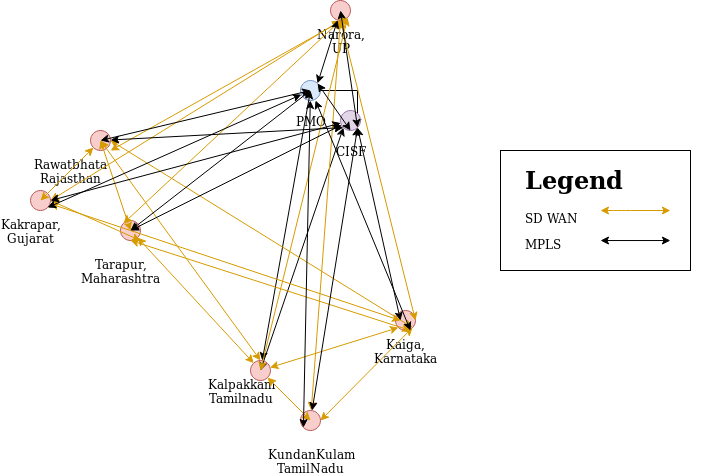
\includegraphics[width=12cm,height=6cm]{ass1.png}
\end{figure}
In India, we have 7 Nuclear power plants. we shall have interconnectivity between each of the power plants, and interconnectivity between CISF, PMO and each of the power plant.

\section{Networking between DAE and other Nuclear Power Plants}
\subsection{Requirement}
The nuclear power plants across India and Department of Atomic Energy offices should be able to get access to specific sections of the power plant and data communication should happen in reliable and secure manner.
\subsection{SD-WAN}
Software defined Wide Area Networking is a method of management and operation of a WAN by decoupling the networking hardware from its control mechanism. This protocol is being chosen mainly because most of the data that needs to be communicated with DAE will be confidential and security is a critical consideration. The disadvantage of this architecture is that due to a lot of rules that needs to be verified for communication, the data transfer will be slower when compared to other WAN technologies. This will not be an issue with respect to our requirement as most of the data that needs to be shared with other DAE and Nuclear power plants is not immediate in nature. Please note that, immediate in this case is few micro seconds. The WAN will not be too slow (few to several minutes) as that will turn out to be a liability in case of emergencies. For example, lately Kudamkulam was infected with a malware and such information needs to be informed to DAE and other power plants. In this case, several minutes delay is not preferred. But SD-WAN at the most only causes a few milliseconds of delay which can be afforded.
\subsubsection{Architecture}
SD-WAN consists of several programmable switches and controllers connected to it. Controller dictates the packet forwarding rule and switches forward the packet according to that rule. In our SD-WAN, we have programmable switches:
\begin{itemize}
	\item At the edge of network gateway acting as a firewall
	\item At edge of each department VLAN for individually being able to forward packets to DAE and nuclear power plants
	\item At the server that collects live data from the sensors protected by another firewall
\end{itemize}
All controllers and fibre optic switches are connected using fibre optic cables.
\begin{figure}[htb]
	\centering
	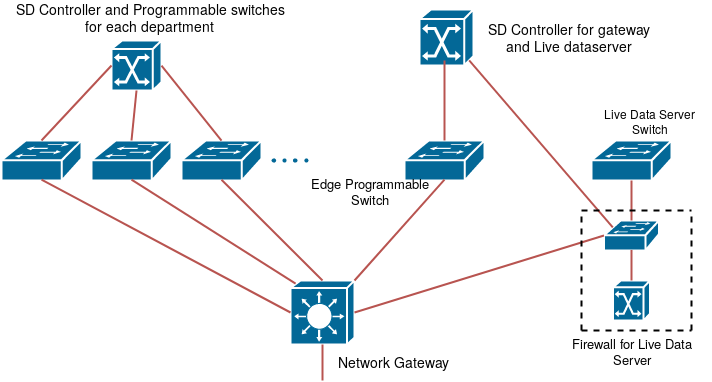
\includegraphics[width=12cm,height=6cm]{sdwan.png}
\end{figure}
All the above shown switches are programmable switches connected to some SD controller. The SD controller is where rules are configured and the switches do the forwarding. There is no requirement for another firewall in the network gateway as the SD WAN devices itself can be configured in such a manner that it does everything a firewall does. There is a separate firewall installed for live data as the number of rules will be very large and might overload the common controller. All rules related to live data filtering to send to DAE office can happen in this firewall.

\subsubsection{Protocol and Device Specifications}
The rules for all SDN devices are configured using \textbf{Cisco Open SDN Controller}. \textbf{Terneray Content Addressable Memory (TCAM)} tables are used to route packet sequences. If flows arrive at a switch, a flow table lookup is performed. Depending on the flow table implementation this is done in a software flow table. In the case when no matching flow is found, a request to the controller for further instructions is sent. This is done using \textbf{Hybrid-mode} which is a combination of two modes: Reactive and Proactive mode.  In reactive mode the controller acts after these requests and creates and installs a rule in the flow table for the corresponding packet if necessary. In proactive mode the controller populates flow table entries for all possible traffic matches possible for this switch in advance. Hybrid mode, follows the flexibility of a reactive mode for a set of traffic and the low-latency forwarding (proactive mode) for the rest of the traffic. \textbf{Cisco's vEdge} routers can be used as switches for SD-WAN. Lanner Incorporated's \textbf{Hybrid TCA 5000} is another option for this.
\section{Wireless Personal Area Network for live data}
It is important to get live updates from inside the nuclear reactor for safety and monitoring and also to control the working of the reactor. Temperature sensors and pressure sensors are used to get live reading of temperature inside the reactor. Movement sensors can also be used to check movement inside the room to control its electricity supply. Since these sensors and its corresponding controllers need to be working all the time, it is important that they have to be power-saving. For this reason, we propose 6LoWPAN devices for IoT.
\begin{figure}[htb]
	\centering
	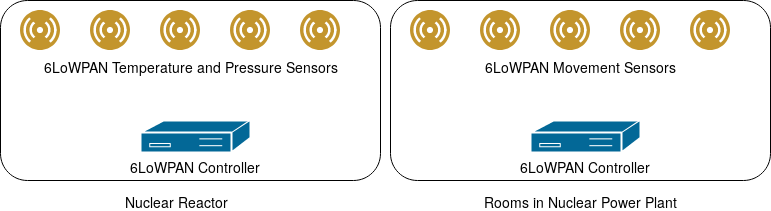
\includegraphics[width=12cm,height=3cm]{wpan_design.png}
\end{figure}
\subsection{Protocol and Device Specifications}
For the Wireless personal area networks we propose \textbf{6LoWPAN} technology. 6LoWPAN stands for IPv6 over Low Powered Wireless Personal Area Networks. 6LoWPAN is a networking technology or adaptation layer that allows IPv6 packets to be carried efficiently within small link layer frames, such as those defined by IEEE 802.15.4. 6LoWPAN is an open standard defined in RFC 6282 by the Internet Engineering Task Force (IETF), the standards body that defines many of the open standards used on the Internet such as UDP, TCP and HTTP to name a few. A powerful feature of 6LoWPAN is that while originally conceived to support IEEE 802.15.4 low-power wireless networks in the 2.4-GHz band, it is now being adapted and used over a variety of other networking media. \textbf{Texas Instruments} make 6LoWPAN temperature sensors, pressure sensors and movement sensors. Its \textbf{CC2538 Powerful Wireless Microcontroller} or \textbf{TIDA-01547} 6LoWPAN controller can be used for data collection and forwarding to specific systems.

\section{Networking between Power Plants and other Organisations}

\subsection{Connectivity between power plant and PMO.(Protocol-TCP)}
The PMO office shall be connected to the power plant in SD WAN configuration. The PMO office can query the server in power plant and can get information from them. However, restriction in access will be provided. Security is the most important parameter when it comes to transfer of information. Thus, IPSec used with ESP.




\subsection{Connectivity between power plant and the CISF(Protocol-TCP)}
The power plant can send emergency information through a secure network to CISF. MPLS used with IPSec. Emergency information eg- hacking attacks, terrorist attacks or endangerment to power plant would be sent to the CISF so that they can send CISF jawans. Thus communication must be swift and secure and reliable. This can be achieved through MPLS. We had also considered if UDP may be a good option since it may be speedier as it doesnot have to indulge in Handshake. However, the benefit may be upto a few milliseconds, which is negligible if we need to send Army personnel to the plant or send any other help.

\subsection{Connectivity between PMO and CISF}
The CISF and PMO can communicate via TCP protocol and MPLS for a more secure and a reliable network. MPLS has a very good QoS.



\begin{figure}[htb]
	\centering
	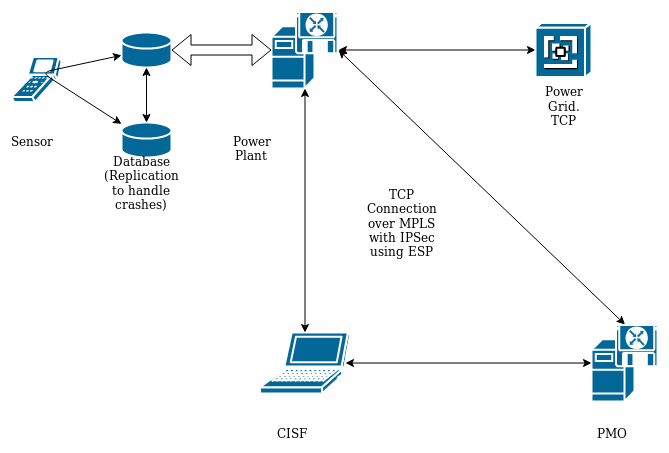
\includegraphics[width=12cm,height=6cm]{ass.png}
\end{figure}
The figure above represents the various interconnectivity of data flow and storage in our system. Data flows from our sensor and is stored in the database as well as is is sent to the controller.
Electricity is supplied to the power grid and the power grid server gives feed back with TCP Protocol and IPSec about how much electricity input it can handle. It can even send warning messages if there may be too much power input. Next we have an interconnectivity between the PMO Office, the CISF and the nuclear power plant. 
\section{Data Storage and Security of the data}
\paragraph{}
Data from the sensors, inputs from the controllers, power grid and logs of packets, details of information shared, power outputs will be amongst the  data that will be stored in a database. 
The database will not be centralised and can be sharded onto different databases. Further, backups will have to be maintained. Storage of the data will be as clear text.
\paragraph{}
Since majority of this data is extremely sensitive, we need to implement high security measures, to ensure that it does not go in the wrong hands.
\subsection{Security Measures:}
\paragraph{}
1. Physical Level security:\paragraph{}
This includes measures like ensuring that unauthorised access to the physical devices in the power plant does not happen. 
Devices that contain sensitive data will be kept in a separate room where only biometrically authenticated person may enter.
\paragraph{}
2. Data shall be stored as clear text in the database, since we want to have minimum amount of latency for critical operations. To ensure security, we need to restrict access based on user privileges. Thus certain privilege levels will have to be defined. The head of the nuclear plant, the head engineers, the engineers, the PMO office and the CIRF will have different privilege levels. Eg. The PMO office dont need to know every detail of the sensor readings, while the head engineer does.
\paragraph{}
3. Encrypted Data flow enforcement
An encrypted data flow creates a virtual private network (VPN) between participating end nodes
by encrypting the data between the nodes. 
Encrypted data flows can be created at the network layer of the communication stack (as
described by the OSI model) or at the transport or application layer.\paragraph{}
The protocol used is the IPSec.
 IPsec is normally used to connect external sites over a wide area network (WAN). It can be configured to operate in transport mode and implemented between two distant power plants or in tunnel mode, which is implemented on a gateway device. \paragraph{}
Remote access can be implemented with the use of VPN appliances that can provide data integrity and confidentiality. For proper network access interrogation, the termination point for a VPN flow
should be at the edge of the protected network. The reason for this termination point is
to allow the data flow to be decrypted and analyzed by additional security devices, such as a
firewall or IDS. This will ensure the VPN is connecting to the proper end point devices within
the protected network and is implementing the proper application. Each authorized VPN should
be documented in the network security policy.
\paragraph{}

4.  Application and User level Security\paragraph{}
a) The workers of the power plant need to login with an ID and a password. \paragraph{}
b) The browsers of the workers can be sandboxed. Various applications can aalso be sandboxed. This will help with preventing zero day attacks, and will thwart attempts of viruses.


\section{Connecting International Bodies}
There is a need for Prime Minister of India (through the Nuclear Power Plant) to make secure international connections to bodies like United Nations and POTUS (President of United States). This may be for various reasons primary of which includes sending data regarding how the nuclear fuel is being used. This is done usually because United Nations want to keep a check of whether nuclear fuel is being used to make illegal weapons. The data should be therefore confidential and data transfer should be highly reliable. Since regular WAN protocols like MPLS, SD-WAN and VSAT only connect within specific geographic location (usually a country), we need to do something else to establish this kind of connection. There are many service providers such as Verizon that provides secure and reliable data transfers internationally. Using this we can establish a secure connection between PMO and United Nations or Nuclear Power Plants and United nations.


\section{Conclusion}
``I always thought something was fundamentally wrong with the universe'' \citep{adams1995hitchhiker}

\bibliographystyle{plain}
\bibliography{references}
\end{document}
